%%%%%%%%%%%%%%%%%%%%%%%%%%%%%%%%%%%%%%%%%%%%%%%%%%%%%%%%%%%%%%%%%%%%%%%%%%%%%%%%
% --------------------------------------------------- ADD APPENDIX (IN CASE) ---
%%%%%%%%%%%%%%%%%%%%%%%%%%%%%%%%%%%%%%%%%%%%%%%%%%%%%%%%%%%%%%%%%%%%%%%%%%%%%%%%
\appendix


\chapter{Detector Overview}

In order to determine the specific \Kr\ activity in the second method, only the data of the detectors that have been turned on during the entire time could be used.
Table \ref{tab:Detector} lists all detectors and shows whether they have continuously recorded data from runs 53 to 92 or from 55 to 92.
In the final analysis, only the data set of runs 55 to 92 was used, as during this time set more detectors have been continuously measuring, which results in a higher exposure ($41.5 \ \unit{kg}\times\unit{yr}$) compared to the alternative ($21.9 \ \unit{kg}\times\unit{yr}$).
\begin{table}
    \centering
	\begin{tabular}{|l|l|c|c||l|l|c|c|}
		\hline
		Channel & Type & 53-92 & 55-92 & Channel & Type & 53-92 & 55-92 \\
		\hline
		0 & BEGe & X & X & 20 & BEGe & X & X \\
		\hline
		1 & BEGe & X & X & 21 & BEGe & X & X \\
		\hline
		2 & BEGe & X & X & 22 & BEGe & X & X \\
		\hline
		3 & BEGe &  & X & 23 & BEGe &  &  \\
		\hline
		4 & BEGe &  & X & 24 & BEGe & X & X \\
		\hline
		5 & BEGe &  &  & 25 & BEGe &  &  \\
		\hline
		6 & BEGe &  &  & 26 & BEGe &  &  \\
		\hline
		7 & BEGe &  &  & 27 & COAX &  &  \\
		\hline
		8 & COAX &  & X & 28 & COAX &  & X \\
		\hline
		9 & COAX &  & X & 29 & COAX & X & X \\
		\hline
		10 & COAX & X & X & 30 & BEGe & X & X \\
		\hline
		11 & BEGe & X & X & 31 & BEGe &  & X \\
		\hline
		12 & BEGe &  & X & 32 & BEGe &  &  \\
		\hline
		13 & BEGe &  &  & 33 & BEGe &  &  \\
		\hline
		14 & BEGe & X & X & 34 & BEGe & &  \\
		\hline
		15 & BEGe &  &  & 35 & BEGe &  &  \\
		\hline
		16 & BEGe &  &  & 36 & COAX &  &  \\
		\hline
		17 & BEGe & X & X & 37 & natural &  &  \\
		\hline
		18 & BEGe &  & X & 38 & natural &  &  \\
		\hline
		19 & BEGe & X & X & 39 & natural &  &  \\
		\hline
	\end{tabular}
	\caption{Detector overview. It indicates which detectors have continuously been switched on during the runs 53-29 or 55-92 by placing an X in the respective box.}
	\label{tab:Detector}
\end{table}
\iffalse
\chapter{Additional Figures}
\label{sec:ResDetermination}


Two calibration spectra have been recorded using different gamma sources at various energies (see figure \ref{fig:Aufloesung})\cite{agostini_background_2017}.
By fitting the two spectra, it was possible to determine two spectral resolution functions for the respective detectors (see equation \ref{equ:BEGeCal} and \ref{equ:COAXCal}).
With these, the resolution and, thus, the full width at half maximum (FWHM) of any gamma line can be determined as a function of the energy.
Using these functions, the resolution of the detectors at the 514 keV line can be determined as $\Delta E_{\mathrm{BEGe}}] =2.26706 \unit{keV}$ for the BEGe and $\Delta E_{\mathrm{COAX}}] = 2.72196 \unit{keV}$ in the COAX detectors.



\begin{equation}
\Delta E_{\mathrm{BEGe}}(E) = 2.35482 \times \sqrt{0.7065+0.00043\times E[\unit{keV}]}
\label{equ:BEGeCal}
\end{equation}

\begin{equation}
\Delta E_{\mathrm{COAX}}(E) = 2.35482 \times \sqrt{1.01314+0.00063\times E[\unit{keV}]}
\label{equ:COAXCal}
\end{equation}
\\
\fi
\iffalse
\begin{figure}
	\centering
	\ifmakefigures%
	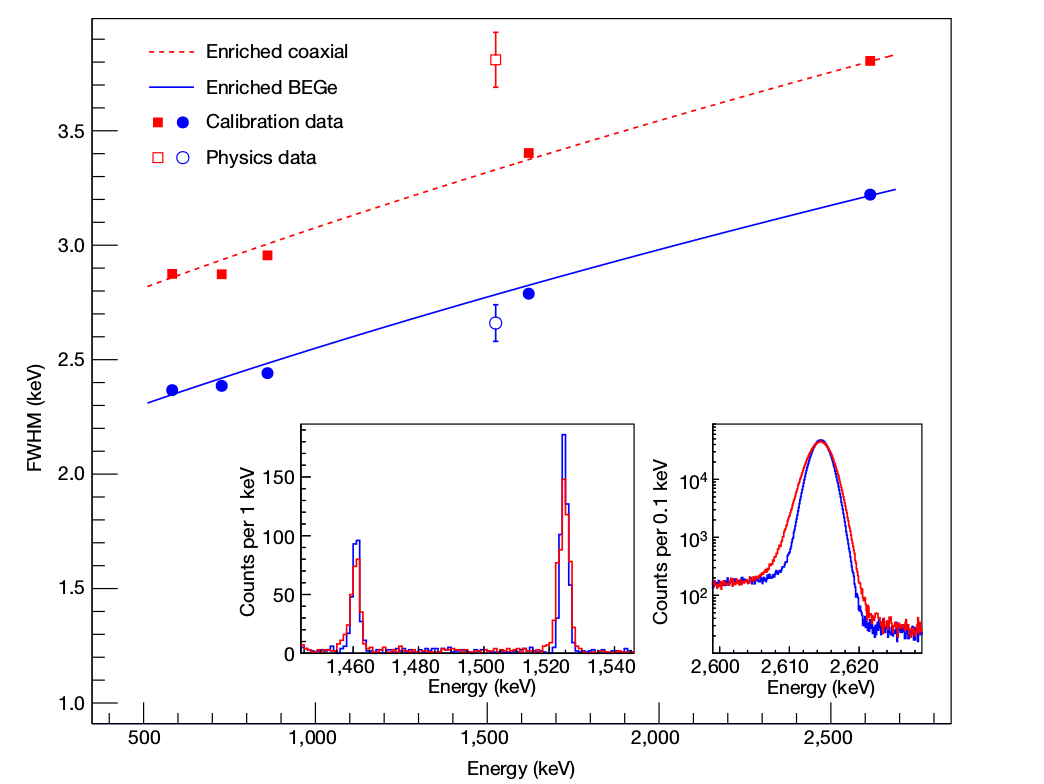
\includegraphics[width=80mm]{./Bilder/Aufloesung.png}
	\fi%
	\caption{
		The full width at half maximum (FWHM) of an investigated gamma line in the respective detectors as a function of the energy of the investigated gamma.
		This value corresponds to the average resolution of the detector type at the respective energy.
		Taken from \cite{agostini_background_2017}.
	}
	\label{fig:Aufloesung}
\end{figure}
\fi
\iffalse
For the fitting process, it is also of interest to know the value of the expected variance $\sigma$ of the Gaussian peak functions.
With the FWHM this can easily be calculated by applying function \ref{equ:sigma}.

\begin{equation}
\sigma (\Delta E) = \frac{\Delta E}{2\sqrt{2\ln2}}
\label{equ:sigma}
\end{equation}

It was therefore possible to calculate $\sigma_{\mathrm{BEGe}} = 0.963 \unit{keV}$ and $\sigma_{\mathrm{COAX}} = 1.156 \unit{keV}$ at an energy of 514 keV.
\fi


% \section{}
% \label{}
